%%%---PREAMBLE---%%%%%%%%%%%%%%%%%%%%%%%%%%%%
\documentclass[oneside,12pt,final]{sty/ucthesis-CA2012}
\pdfoutput=1

%--- Packages ---------------------------------------------------------
\usepackage[lofdepth,lotdepth,caption=false]{subfig}
\usepackage{fancyhdr}
\usepackage{hyperref}
\usepackage{amsmath, amssymb, graphicx}
\usepackage{xspace}
\usepackage{braket}
\usepackage{color}
\usepackage{setspace}
\usepackage{bibentry}
%\usepackage{subfigure} (Subfigure package clashes with another package)

%---New Definitions and Commands------------------------------------------------------
\def\p{\partial}
\def\im{\mrm{im}}
\def\Tr{\mrm{Tr}}
\def\Z{\mbb{Z}}
\def\R{\mbb{R}}
\def\C{\mbb{C}}
\def\half{\frac{1}{2}}
\def\filler{\phantom{fillerfillerfiller}}
\newcommand{\be}{\begin{equation}}
\newcommand{\ee}{\end{equation}}
\newcommand{\mbb}[1]{\mathbb{#1}}
\newcommand{\mrm}[1]{\mathrm{#1}}
\newcommand{\mcal}[1]{\mathcal{#1}}
\newcommand{\mbf}[1]{\mathbf{#1}}
\newcommand{\ph}[1]{\phantom{#1}}
\newcommand{\udten}[3]{#1^{#2}_{\ph{#2}#3}}
\newcommand{\duten}[3]{#1^{\ph{#2}#3}_{#2}}
\newcommand{\pd}[2]{\frac{\p#1}{\p#2}}
\newcommand{\D}[2]{\frac{d#1}{d#2}}
\newcommand{\sthirteen}{\ensuremath{\sqrt{\mathrm{s}}=13~\mathrm{TeV}}\xspace}
\newcommand{\ifb}{fb\ensuremath{{}^{-1}}}

%---Set Margins ------------------------------------------------------
\setlength\oddsidemargin{0.25 in} \setlength\evensidemargin{0.25 in} \setlength\textwidth{6.25 in} \setlength\textheight{8.50 in}
\setlength\footskip{0.25 in} \setlength\topmargin{0 in} \setlength\headheight{0.25 in} \setlength\headsep{0.25 in}

%%%---DOCUMENT---%%%%%%%%%%%%%%%%%%%%%%%%%%%%
\begin{document}

%=== Preliminary Pages ============================================
\begin{frontmatter}
	%%%%%%%%%%%%%%%%%%%%%%%%%%%
% TITLE PAGE INFORMATION %
%%%%%%%%%%%%%%%%%%%%%%%%%%%


\title{Methodological observation of the sociometrical behavior tendencies of pre-maturated isolates}

\author{David McAlister Barry}

%%%%%%%%%%%%%%%%%%%%%%%%%%%%%%%%%%
% DECLARATIONS FOR FRONT MATTER %
%%%%%%%%%%%%%%%%%%%%%%%%%%%%%%%%%%
\report{Dissertation} \degree{Doctor of Philosophy} \degreemonth{Month} \degreeyear{2018}
\defensemonth{March} % should be one of the following: March, 
\defenseyear{2018}

\chair{Professor Charles McThornbody}  % this is your advisor
\othermemberA{Professor Russell Hammond} % This is a member of your committee 
\othermemberB{Professor Alfred Alfredo} % This is a member of your committee 
\othermemberC{Professor Jackmerius Tacktheritrix} % This is a member of your committee (if your department requires 4 members)
\numberofmembers{4} % should match the number of entries above (chair + othermembers)

\field{Electrical and Computer Engineering}
\campus{Santa Barbara}


%\title{{ University of California \\ Santa Barbara} \linebreak \\  Ph.D. Dissertation}
%\author{Tom\'as Andrade}
%\date{2012}

	\maketitle
	\approvalpage
	\copyrightpage
	% \begin{dedication}

\bigskip

${}$ \\

\bigskip

${}$ \\

\bigskip

${}$ \\

\bigskip

\begin{center}
\begin{Large}
Dedication here
\end{Large}
\end{center}


\end{dedication} %comment out if you don't want a dedication
	\begin{acknowledgements}

Acknowledgements Here.  

\end{acknowledgements} 
	\begin{vitae}
\addcontentsline{toc}{chapter}{Curriculum Vitae}

\begin{vitaesection}{Education}
\vspace{-0.1cm}
\item [2019] Ph.D. in Physics (Expected), University of California, Santa Barbara.
\item [2017] M.Sc. in Physics, University of California, Santa Barbara.
\item [2014] B.Sc. in Physics, Texas A\&M University, College Station, TX.
\end{vitaesection}

\textbf{Publications}

% \nobibliography*
% \begin{itemize}
%     \item \bibentry{GAN:LHC2019} % http://inspirehep.net/record/1714018
%     \item \bibentry{CMS:myTOPRun2PAS} % http://inspirehep.net/record/1726177
%     \item \bibentry{CMS:mySUSRun2PAS} % http://inspirehep.net/record/1726691
%     \item \bibentry{CMS:myTOP2016} % http://inspirehep.net/record/1633423
%     \item \bibentry{CMS:mySUS2016} % http://inspirehep.net/record/1594731
% \end{itemize}


    \begin{itemize}
        \item B. Hashemi, N. Amin, K. Datta, D. Olivito, and M. Pierini, \textit{LHC analysis-specific datasets with Generative Adversarial Networks} [\href{https://arxiv.org/abs/1901.05282}{arXiv:1901.0528}] \textbf{In progress}
        \item CMS Collaboration, \textit{Search for standard model production of four top quarks in final states with same-sign and multiple leptons in proton-proton collisions at \sthirteen} 
            [\href{http://inspirehep.net/record/1726177}{PAS TOP-18-003}] \textbf{In progress}
        \item CMS Collaboration, \textit{Search for physics beyond the standard model in events with two same-sign leptons or at least three leptons and jets in proton-proton collisions at \sthirteen} 
            [\href{http://inspirehep.net/record/1726691}{PAS SUS-19-008}] \textbf{In progress}
        \item CMS Collaboration, \textit{Search for standard model production of four top quarks with same-sign and multilepton final states in proton-proton collisions at \sthirteen},
            \textit{Eur. Phys. J.} \textbf{C78} (2018) 
            [\href{https://arxiv.org/abs/1710.1061}{arXiv:1710.1061}]
        \item CMS Collaboration, \textit{Search for physics beyond the standard model in events with two leptons of same sign, missing transverse momentum, and jets in proton-proton collisions at \sthirteen}
            \textit{Eur. Phys. J.} \textbf{C77} (2017) 
            [\href{https://arxiv.org/abs/1704.07323}{arXiv:1704.07323}]
    \end{itemize}

\end{vitae}

	\begin{abstract}
\addcontentsline{toc}{chapter}{Abstract}

Two related searches for Standard Model and beyond the Standard Model physics
    with a final state containing a pair of same-charged leptons and jets are
    performed using a sample of \sthirteen data corresponding to an integrated
    luminosity of 137~\ifb, collected by the CMS detector between 2016 and
    2018. The first inclusive search observes no excess above the Standard
    Model and thus places constraints on R-parity violating and R-parity
    conserving supersymmetric models with pair production of gluinos and
    squarks.  Gluino masses are excluded up to 2.1 TeV, while top and bottom
    squarks are excluded up to 0.9 TeV.  The second search measures the
    cross-section of the production of four top quarks within the Standard
    Model using both cut-based and multivariate approaches.  The observed
    (expected) significance of the multivariate approach is 2.6 (2.7) standard
    deviations, with a measured cross-section of $12.6^{+5.8}_{-5.2}$ fb,
    consistent with the Standard Model prediction of $12.0^{+2.2}_{-2.5}$ fb.
    These results are translated into constraints on the Yukawa coupling of the
    top quark, as well as constraints on heavy scalar or pseudoscalar
    production in a type II 2HDM scenario.

%\abstractsignature
\end{abstract}



	\tableofcontents
\end{frontmatter}

\begin{mainmatter}

%---Set Headers and Footers ------------------------------------------------------
\pagestyle{fancy}
\renewcommand{\chaptermark}[1]{\markboth{{\sf #1 \hspace*{\fill} Chapter~\thechapter}}{} }
\renewcommand{\sectionmark}[1]{\markright{ {\sf Section~\thesection \hspace*{\fill} #1 }}}
\fancyhf{}

\makeatletter \if@twoside \fancyhead[LO]{\small \rightmark} \fancyhead[RE]{\small\leftmark} \else \fancyhead[LO]{\small\leftmark}
\fancyhead[RE]{\small\rightmark} \fi

\def\cleardoublepage{\clearpage\if@openright \ifodd\c@page\else
  \hbox{}
  \vspace*{\fill}
  \begin{center}
    This page intentionally left blank
  \end{center}
  \vspace{\fill}
  \thispagestyle{plain}
  \newpage
  \fi \fi}
\makeatother
\fancyfoot[c]{\textrm{\textup{\thepage}}} % page number
\fancyfoot[C]{\thepage}
\renewcommand{\headrulewidth}{0.4pt}

\fancypagestyle{plain} { \fancyhf{} \fancyfoot[C]{\thepage}
\renewcommand{\headrulewidth}{0pt}
\renewcommand{\footrulewidth}{0pt}}

%=== Introduction ============================================
\chapter{Introduction}

\begin{section}{Info}
Some facts

\begin{itemize}

\item Standard model missing some stuff
\item LHC smashes protons together very fast
\item CMS detector is very big
\item Analyze CMS data to find stuff beyond the standard model (e.g., SUZY)
\item Did not find anything

\end{itemize}
\end{section}

% \begin{figure}[t]
% \centerline{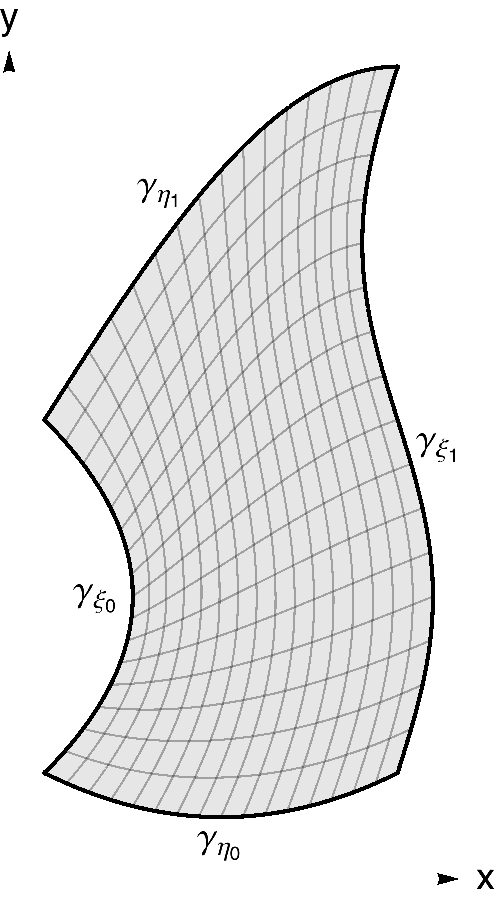
\includegraphics[width=.35\textwidth]{figs/testfig1.pdf}
% \hspace{1cm}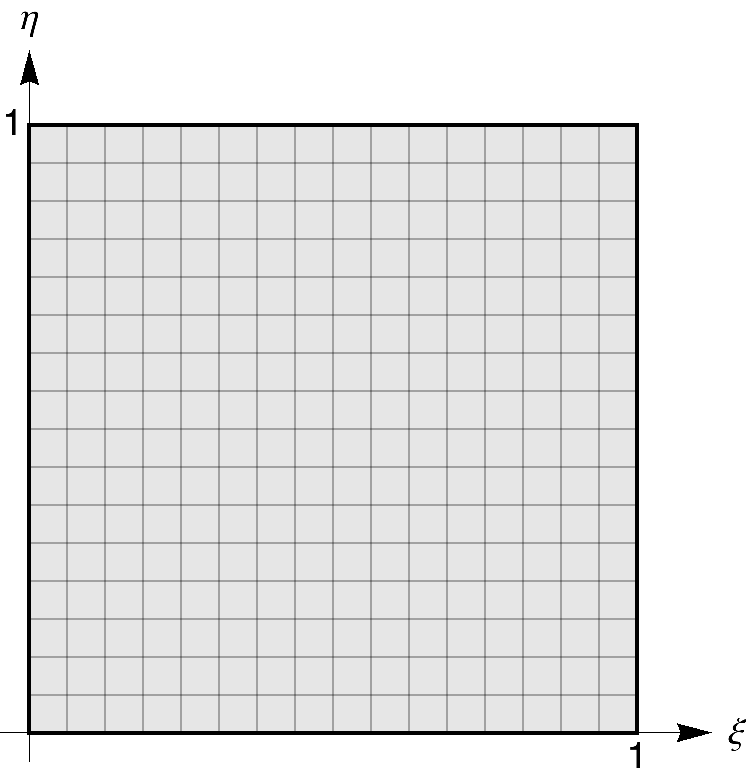
\includegraphics[width=.45\textwidth]{figs/testfig2.pdf}}
% \caption{Figure Captions.}
% \label{fig:label}
% \end{figure}

%=== Appendix ============================================
\appendix

\dsp

\chapter{Appendix Title}{\label{appendix:a}}
\begin{section}{Section Title}
Feed me later, please
\end{section}

\end{mainmatter}

%----- Bibliography ----------------
\ssp
\bibliographystyle{sty/JHEP3}
\bibliography{bib/thesis}

\end{document} 
